% \documentclass[9pt,t]{beamer}
\usefonttheme{professionalfonts}
\usefonttheme{serif}
\PassOptionsToPackage{pdfpagemode=FullScreen}{hyperref}
\PassOptionsToPackage{usenames,dvipsnames}{color}
% \DeclareGraphicsRule{*}{mps}{*}{}
\usepackage{linalgjh}
\usepackage{present}
\usepackage{directories}  % Define \jcdir, \jcmpdir, etc.
\usepackage{xr}\externaldocument{\jcdir jc2} % read refs from .aux file
\usepackage{catchfilebetweentags}
\usepackage{etoolbox} % from http://tex.stackexchange.com/questions/40699/input-only-part-of-a-file-using-catchfilebetweentags-package
\makeatletter
\patchcmd{\CatchFBT@Fin@l}{\endlinechar\m@ne}{}
  {}{\typeout{Unsuccessful patch!}}
\makeatother

\usepackage{polynom}  % for polynomial long division

\mode<presentation>
{
  \usetheme{boxes}
  \setbeamercovered{invisible}
  \setbeamertemplate{navigation symbols}{} 
}
\addheadbox{filler}{\ }  % create extra space at top of slide 
\hypersetup{colorlinks=true,linkcolor=blue} 

\title[Angles and Eigenvectors] % (optional, use only with long paper titles)
{Angles and Eigenvectors}

\author{\textit{Linear Algebra} \\ {\small Jim Hef{}feron}}
\institute{
  \texttt{https://hefferon.net/linearalgebra}\\[0.25ex]
  \texttt{http://joshua.smcvt.edu/linearalgebra}
}
\date{}


\subject{Eigenvectors}
% This is only inserted into the PDF information catalog. Can be left
% out. 

\begin{document}
\begin{frame}
  \titlepage
\end{frame}


\section{Lines transform to lines}
%..........
\begin{frame}{Lines go to lines}
Consider a real space transformation
$\map{t}{\Re^n}{\Re^n}$.
A defining property of linear maps is that 
$t(r\cdot\vec{v})=r\cdot t(\vec{v})$.

In a real space $\Re^n$ a line through the origin is a set 
$\set{r\cdot \vec{v}\suchthat r\in\Re}$. 
So $t$'s action 
\begin{equation*}
  r\cdot\vec{v}\mapsunder{t} r\cdot t(\vec{v})
\end{equation*}
is to send members of the line $\set{r\cdot \vec{v}\suchthat r\in\Re}$
in the domain to members of the line
$\set{s\cdot t(\vec{v})\suchthat s\in\Re}$
in the codomain. 

Thus, lines through the origin 
transform to lines through the origin.
Further, the action of~$t$ is determined by its effect $t(\vec{v})$
on any
nonzero vector element of the domain line.
\end{frame}
\begin{frame}
\ex
Consider the line~$y=2x$ in the plane 
\begin{equation*}
  \set{r\cdot\colvec{1 \\ 2}\suchthat r\in\Re}
\end{equation*}
and this transformation $\map{t}{\Re^2}{\Re^2}$ of the plane.
\begin{equation*}
  \colvec{x \\ y}
  \mapsto
  \colvec{x+3y \\ 2x+4y}
\end{equation*}
The map's effect on any vector in the line is easy to compute.
\begin{equation*}
  \vec{v}=\colvec{1 \\ 2}\mapsunder{t}\colvec{7 \\ 10}
\end{equation*}
The scalar multiplication property in the definition of linear map 
$t(r\cdot\vec{v})=r\cdot t(\vec{v})$
imposes a uniformity on $t$'s action:~it 
has twice the effect on $2\vec{v}$, three times the
effect on $3\vec{v}$, etc.
\begin{equation*}
  \colvec{2 \\ 4}\mapsunder{t}\colvec{14 \\ 20}
  \qquad
  \colvec{-3 \\ -6}\mapsunder{t}\colvec{-21 \\ -30}
  \qquad
  \colvec{r \\ 2r}\mapsunder{t}\colvec{7r \\ 10r}
\end{equation*}
In short: the action of $t$ on any  nonzero $\vec{v}$
determines its action on any other vector $r\vec{v}$
in the line $\spanof{\vec{v}}$.
\end{frame}


\begin{frame}
  \frametitle{Pick one, any one}
Every plane vector is in some line through the origin
so to understand what $\map{t}{\Re^2}{\Re^2}$ does to 
plane elements it suffices to 
understand what it does to lines through the origin. 
By the prior slide, to understand what $t$ does to a line through the 
origin it suffices to understand what it does to a single nonzero
vector in that line.

\pause
So one way to understand a transformation's action is to take
a set containing one nonzero vector from each line through the origin,
and describe where the transformation maps the elements of that set.

A natural set with one nonzero element from each line through the
origin is the upper half unit circle (we will explain the colors below).
\begin{equation*}
  \set{\colvec{x \\ y}
       =\colvec{\cos(t) \\ \sin(t)}
         \suchthat 
         0\leq t<\pi}
  \qquad
  \vcenteredhbox{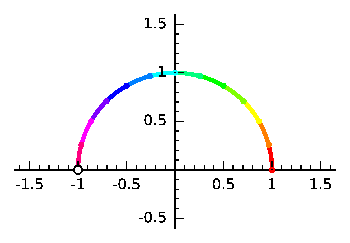
\includegraphics[scale=0.75]{graphics/five_ii_a_unithalfcircle.pdf}}  
\end{equation*}  
\end{frame}




\section{Angles in plane transformations}
% =============================================
\begin{frame}{Angles}
\ex
This plane transformation.
\begin{equation*} 
  \colvec{x \\ y} \mapsto \colvec{2x \\ 2x+2y}
\end{equation*}
is a skew.
\begin{equation*}
  \vcenteredhbox{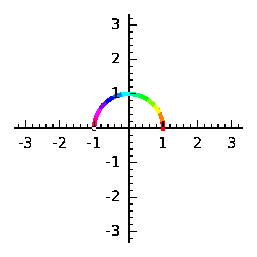
\includegraphics[scale=.75]{graphics/five_ii_a_skew1.pdf}}
  \quad\rightarrow\quad
  \vcenteredhbox{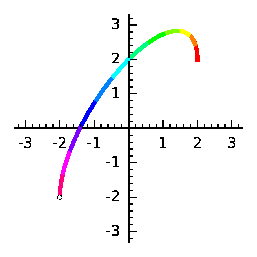
\includegraphics[scale=.75]{graphics/five_ii_a_skew2.pdf}}
\end{equation*}
\pause
As we move through the unit half circle on the left, the 
transformation has varying effects on the vectors.
The dilation vary,
that is, different vectors get their length multiplied by different factors, 
and they are turned through varying angles.
The next slide gives examples.  
\end{frame}
\begin{frame}
The prior slide's vector from the left shown in red
is dilated by a factor of $2\sqrt{2}$ and rotated counterclockwise 
by $\pi/4\approx0.78$~radians.
\begin{equation*}
  \colvec{1 \\ 0}\mapsto \colvec{2 \\ 2}
  \qquad
  \vcenteredhbox{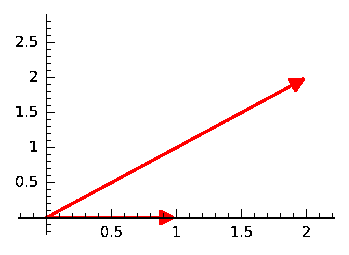
\includegraphics[scale=.75]{graphics/five_ii_a_skew3.pdf}}
\end{equation*}
The orange vector
is dilated by a factor of $2\sqrt{\cos^2(\pi/6)+1}=\sqrt{7}$ and rotated 
by about $0.48$~radians.
\begin{equation*}
  \colvec{\cos(\pi/6) \\ \sin(\pi/6)}\mapsto \colvec{2\cos(\pi/6) \\ 2\cos(\pi/6)+2\sin(\pi/6)}
  \qquad
  \vcenteredhbox{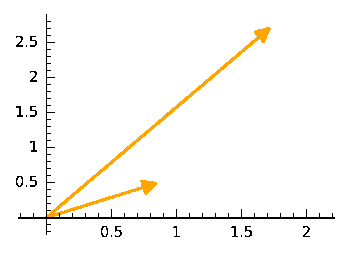
\includegraphics[scale=.75]{graphics/five_ii_a_skew4.pdf}}
\end{equation*}
\end{frame}

\begin{frame}
On the graph below the horizontal axis is the angle of 
a vectors from the upper half unit circle,
while the vertical axis is
the angle through which that vector is rotated.  
\begin{equation*}
  \colvec{x \\ y}\mapsto \colvec{2x \\ 2x+2y}
  \qquad
  \vcenteredhbox{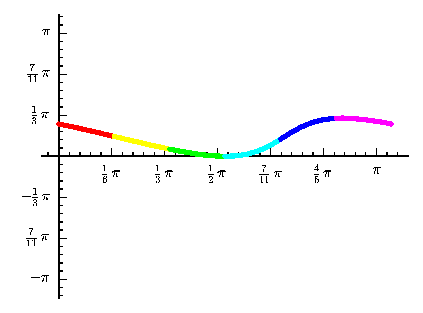
\includegraphics{graphics/five_ii_a_skew5.pdf}}
\end{equation*}
The rotation angle of interest is~$0$~radians, here achieved 
by some green vector.
\end{frame}


\begin{frame}{Definition}
A vector that is rotated through an angle of $0$~radians or of $\pi$~radians,
while being dialated by a nonzero factor, is an \alert{eigenvector}.
The factor by which it is dilated is the \alert{eigenvalue}.    
\end{frame}



%................
% diagonal
\begin{frame}
\ex
The plane transformation
\begin{equation*} 
  \colvec{x \\ y} \mapsto \colvec{-x \\ 2y}
\end{equation*}
represented with respect to the standard bases by a diagonal matrix
\begin{equation*}
  \begin{mat}
    -1  &0  \\
     0  &2
  \end{mat}
\end{equation*}
has this simple action on the upper half unit circle.
\begin{equation*}
  \vcenteredhbox{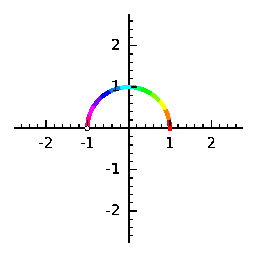
\includegraphics[scale=.75]{graphics/five_ii_a_diagonal1.pdf}}
  \quad\rightarrow\quad
  \vcenteredhbox{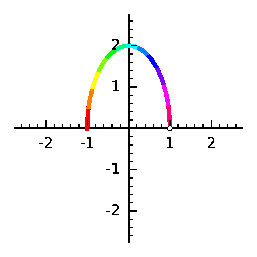
\includegraphics[scale=.75]{graphics/five_ii_a_diagonal2.pdf}}
\end{equation*}
\end{frame}
\begin{frame}
This
plots the angle of each vector in the upper half unit circle
against the angle through which it is rotated.  
\begin{equation*}
  \colvec{x \\ y}\mapsto \colvec{-x \\ 2y}
  \qquad
  \vcenteredhbox{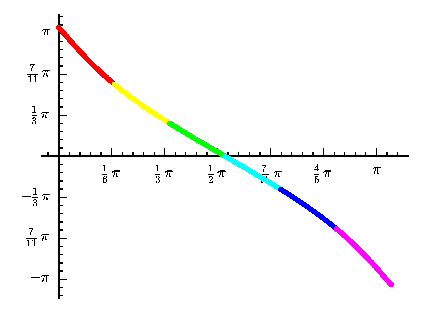
\includegraphics{graphics/five_ii_a_diagonal3.pdf}}
\end{equation*}
One vector gets zero rotation, the vector with $x=0$.
\end{frame}



%................
% generic
\begin{frame}
\ex
This generic plane transformation
\begin{equation*} 
  \colvec{x \\ y} \mapsto \colvec{x+2y \\ 3x+4y}
\end{equation*}
has this action on the upper half unit circle.
\begin{equation*}
  \vcenteredhbox{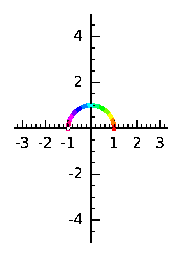
\includegraphics[scale=.75]{graphics/five_ii_a_generic1.pdf}}
  \quad\rightarrow\quad
  \vcenteredhbox{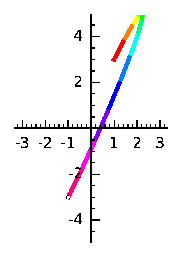
\includegraphics[scale=.75]{graphics/five_ii_a_generic2.pdf}}
\end{equation*}
\end{frame}
\begin{frame}
Plotting the angle of each vector in the upper half unit circle
against the angle through which it is rotated  
\begin{equation*}
  \colvec{x \\ y}\mapsto \colvec{x+2y \\ 3x+4y}
  \qquad
  \vcenteredhbox{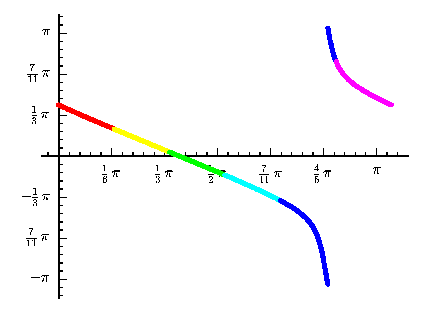
\includegraphics{graphics/five_ii_a_generic3.pdf}}
\end{equation*}
gives that one vector gets a rotation of $0$~radians, while another
gets a rotation of $\pi$~radians.
\end{frame}



%...........................
% \begin{frame}g
% \ExecuteMetaData[../gr3.tex]{GaussJordanReduction}
% \df[def:RedEchForm]
% 
% \end{frame}
\end{document}

Orange vector calculations
sage: 2*((cos(pi/6))^2+1)^(1/2)
sqrt(7)
sage: v=vector(RR,[cos(pi/6), sin(pi/6)])
sage: v
(0.866025403784439, 0.500000000000000)
sage: M=matrix(RR, [[2,0], [2,2]])
sage: M
[ 2.00000000000000 0.000000000000000]
[ 2.00000000000000  2.00000000000000]
sage: M=matrix(RR, [[2,2], [0,2]])
sage: M
[ 2.00000000000000  2.00000000000000]
[0.000000000000000  2.00000000000000]
sage: w=v*M
sage: w
(1.73205080756888, 2.73205080756888)
sage: arccos((w*v)/(w.norm()*v.norm()))
0.482170608511459
